\chapter{Analysis}

\section{Introduction}
My chosen client is Michael Seamark; He is fairly experienced with working with computer systems and mainly uses a laptop to assist with his job and to surf the internet. However, he also uses an iPhone to check his emails and keep in contact with people through social networking sites.

\subsection{Define the current system}
Michael has requested that I produce a metering system which monitors gas, water and electricity consumption with several graphical outputs to represent the use and any possible savings with a way to convert between units. It should be able indicate the current cost for the consumption and predict future costs. Currently, Michael relies on the monthly bills to give him the information on his consumption of electricity, gas and water and then he has to work out any savings, calculate future costs and convert to other units if needed manually.

\subsection{Describe the problems}
One problem with the current system that Michael is using is that he cannot get the consumption of gas or electricity until the end of the month which means that he cannot check the cost of what he has used until the end of the month in which case the cost could have gone up significantly. In addition to that, the method he has to work out current spendings and future savings is inefficient and more prone to mistakes because he is calculating it manually and therefore can get values wrong or misread values from the bill 

\subsection{Section appendix}
\subsubsection{Client Interview}
\begin{enumerate}
	\item What is the proposed system required to do?
It needs to monitor energy used.you want it to monitor gas electricity accurately and be able to display the raw data in various ways eg charts so consumer can see easily what energy is being used. It will also need to calculate an average consumption for each month, 6 months and year and be able to cope with varying amounts of raw data stored in multiple units and calculate an average cost per month to calculate future costs based on the recent price and average consumption

	\item What are the problems with the current way of doing things?
The current system only monitors gas and electricity consumption and prices per month but not water and can only do one at a time so is inefficient. It is also not possible to get a reading before the month is over

	\item What data is currently recorded?
Currently only monthly gas and electricity consumption and averages for the consumption and price per month

	\item What data will the proposed system need to record?
The proposed system will need to take data on the amount of gas, electricity and water consumed per month and store. In addition to this the system will need to store averages of each for up to the past year along with prices for each month, 6 months and year and an average price for the past few months so that a prediction can be made on the cost for the coming month

	\item How will the data be recieved?
The consumption will be taken in real time and incremented onto the use for the month and the data will be stored onto a database and each month a new count will be taken along with an average price per unit of gas, electricity and water respectively

	\item What processes are performed by the current system?
The processes done by the current system are gathering daily electricity and gas consumption and adding it onto the monthly tallys, calculating a price for the past month based on the average cost per unit, calculate an average price of the past few months and calculate a predicted price for the next month

	\item What processes will the new system be required to do?
The new system will need to be able to gather daily electricity, gas and water consumption and increment it onto the monthly tallys for each one, calculate a current price of each based on the average price per unit, calculate an average price of each for the past few months, calculate the average consumption for the past few months and calculate a predicted price for the next month based on average monthly consumption on each for the past few months and average price for the past few months


	\item What algorithms do these processes use?
The current price will use an algorithm which takes the current average cost per unit for gas, electricity and water and multiply the costs by their current consumption values for each.
The average consumption will use an algorithm which calculates the sum of gas consumption for the past few months, the electricity consumption for the past few months and water consumption for the past few months and divide those sums by how many months the average taken data from. 
The average price will use an algorithm similar to the one for the average consumption but it will use values for the prices of each for the past few months rather than consumption

	\item Which processes should be executed manually?
All processes should be automated rather than be done manually

	\item What are the inputs to the current system?
The current system takes inputs for consumption for gas and electricity each day and average unit prices

	\item What inputs are required for the proposed system?
The proposed system will need to take inputs for gas, electricity and water consumption in real time and average unit prices

	\item What are the outputs from the current system?
The current system outputs an average consumption for gas and electricity for the past few months, a price for the past month for each, an average price for the past few months for each and a predicted price for the next month for each

	\item What outputs will be required from the proposed system?
The proposed system will output average consumptions for gas, electricity and water over the past few months, a price for the past month for gas, electricity and water, average costs for gas, electricity and water over the past few months, a predicted price for the following month for gas, electricity and water

\end{enumerate}

\section{Investigation}

\subsection{The current system}

\subsubsection{Data sources and destinations}
\begin{center}
\begin{tabular}{|l|l|l|l|}
	\hline
	\textbf{Source} & \textbf{Data} & \textbf{Example Data} & \textbf{Destination} \\ \hline
	Bill & Gas consumption data & Gas consumption for past month & Notebook \\ \hline
	Bill & Electricity consumption data & Electricity consumption for past month & Notebook \\ \hline
	Bill & Average price per unit for gas & 1.18 pounds/kWh & Notebook \\ \hline
 	Bill & Average price per unit for electricity & 1.34 pounds/kWh & Notebook \\ \hline
\end{tabular}
\label{tab:Data sources and destinations for the current system}
\end{center}

\subsubsection{Algorithms}
\begin{algorithm}[H]
	\caption{Price of gas consumption for the past month}
\begin{algorithmic}[H]
\SET{$gas\_price$}{$0$}
\RECEIVE{$total\_gas\_consumption$}
\RECEIVE{$average\_price\_per\_unit$}
\SET{$gas\_price$}{$total\_gas\_consumption * average\_price\_per\_unit$}
\SEND{$gas\_price$}
\end{algorithmic}
\end{algorithm}

\begin{algorithm}[H]
	\caption{Price of electricity consumption for the past month}
\begin{algorithmic}[H]
\SET{$electricity\_price$}{$0$}
\RECEIVE{$total\_electricity\_consumption$}
\RECEIVE{$average\_price\_per\_unit$}
\SET{$electricity\_price$}{$total\_electricity\_consumption * average\_price\_per\_unit$}
\SEND{$electricity\_price$}
\end{algorithmic}
\end{algorithm}

\begin{algorithm}[H]
	\caption{Average price of gas consumption for the past few months}
\begin{algorithmic}[H]
\SET{$average\_monthly\_price$}{0}
\SET{$total\_price$}{0}
\SEND{$"How\ many\ months\ would\ you\ like\ to\ get\ an\ average\ for?"$}
\RECEIVE{$amount\_of\_months$}
\For{$count$}{$amount\_of\_months$}
	\RECEIVE{$gas\_price$}
	\SET{$total\_price$}{$total\_price + gas\_price$}
\EndFor
\SET{$average\_monthly\_price$}{$total\_price / amount\_of\_months$}
\SEND{$average\_monthly\_price$}
\end{algorithmic}
\end{algorithm}

\begin{algorithm}[H]
	\caption{Average gas consumption for the past few months}
\begin{algorithmic}[H]
\SET{$average\_monthly\_consumption$}{0}
\SET{$total\_consumption$}{0}
\SEND{$"How\ many\ months\ would\ you\ like\ to\ get\ an\ average\ for?"$}
\RECEIVE{$amount\_of\_months$}
\For{$count$}{$amount\_of\_months$}
	\RECEIVE{$gas\_consumption$}
	\SET{$total\_consumption$}{$total\_consumption + gas\_consumption$}
\EndFor
\SET{$average\_monthly\_consumption$}{$total\_consumption / amount\_of\_months$}
\SEND{$average\_monthly\_price$}
\end{algorithmic}
\end{algorithm}

\begin{algorithm}[H]
	\caption{Average price of electricity consumption for the past few months}
\begin{algorithmic}[H]
\SET{$average\_monthly\_price$}{0}
\SET{$total\_price$}{0}
\SEND{$"How\ many\ months\ would\ you\ like\ to\ get\ an\ average\ for?"$}
\RECEIVE{$amount\_of\_months$}
\For{$count$}{$amount\_of\_months$}
	\RECEIVE{$electricity\_price$}
	\SET{$total\_price$}{$total\_price + electricity\_price$}
\EndFor
\SET{$average\_monthly\_price$}{$total\_price / amount\_of\_months$}
\SEND{$average\_monthly\_price$}
\end{algorithmic}
\end{algorithm}

\begin{algorithm}[H]
	\caption{Average electricity consumption for the past few months}
\begin{algorithmic}[H]
\SET{$average\_monthly\_consumption$}{0}
\SET{$total\_consumption$}{0}
\SEND{$"How\ many\ months\ would\ you\ like\ to\ get\ an\ average\ for?"$}
\RECEIVE{$amount\_of\_months$}
\For{$count$}{$amount\_of\_months$}
	\RECEIVE{$electricity\_consumption$}
	\SET{$total\_consumption$}{$total\_consumption + electricity\_consumption$}
\EndFor
\SET{$average\_monthly\_consumption$}{$total\_consumption / amount\_of\_months$}
\SEND{$average\_monthly\_price$}
\end{algorithmic}
\end{algorithm}

\begin{algorithm}[H]
	\caption{Predicted gas consumption price for the coming months}
\begin{algorithmic}[H]
\SET{$predicted\_cost$}{0}
\RECEIVE{$average\_gas\_consumption$}
\RECEIVE{$average\_cost\_per\_unit$}
\SET{$predicted\_cost$}{$average\_gas\_consumption * average\_cost\_per\_unit$}
\SEND{$predicted\_cost$}
\end{algorithmic}
\end{algorithm}

\begin{algorithm}[H]
	\caption{Predicted electricity consumption price for the coming months}
\begin{algorithmic}[H]
\SET{$predicted\_cost$}{0}
\RECEIVE{$average\_electricity\_consumption$}
\RECEIVE{$average\_cost\_per\_unit$}
\SET{$predicted\_cost$}{$average\_electricity\_consumption * average\_cost\_per\_unit$}
\SEND{$predicted\_cost$}
\end{algorithmic}
\end{algorithm}

\subsubsection{Data flow diagram}
\begin{figure}[H]
    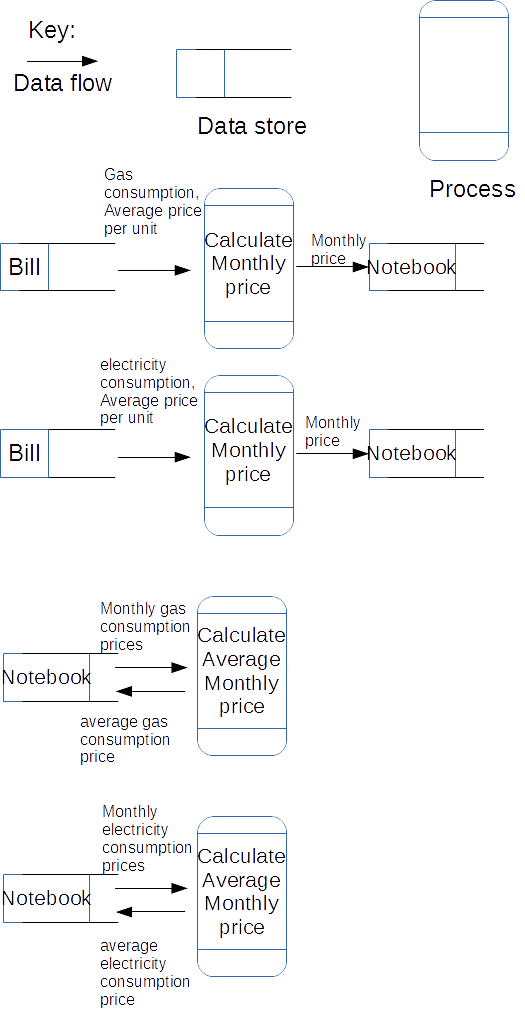
\includegraphics[width=\textwidth]{./dataflowdiagrams1.png}
    \caption{data flow diagrams} \label{fig:dataflowdiagrams}
\end{figure}

\begin{figure}[H]
    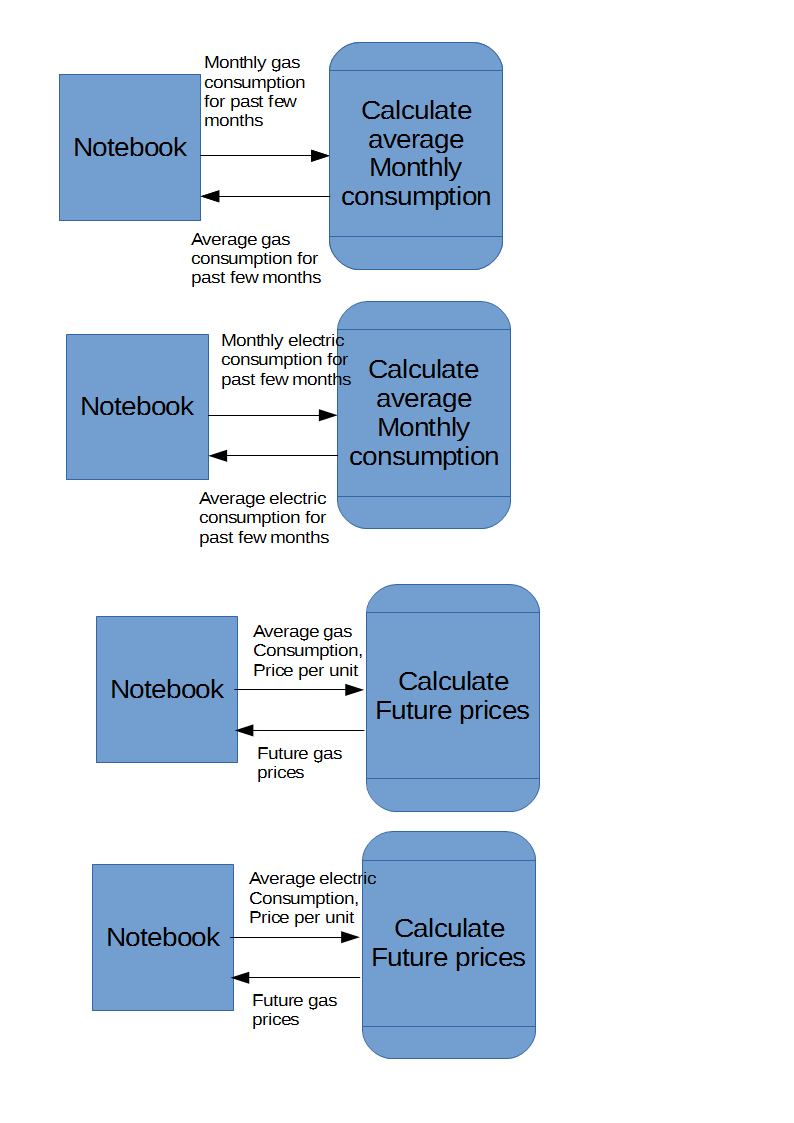
\includegraphics[width=\textwidth]{./dataflowdiagrams2.png}
    \caption{data flow diagrams} \label{fig:dataflowdiagrams}
\end{figure}

\subsubsection{Input Forms, Output Forms, Report Formats}

\subsection{The proposed system}
\begin{center}
\begin{tabular}{|l|l|l|l|}
	\hline
	\textbf{Source} & \textbf{Data} & \textbf{Example Data} & \textbf{Destination} \\ \hline
	gas meter & gas consumption data & gas consumption & database \\ \hline
 	electricity meter & electric consumption data & electric consumption & database \\ \hline
	water meter & water consumption data & water consumption & database \\ \hline
	User input & Average price per unit for gas & 1.18 pounds/kWh & database \\ \hline
 	User input & Average price per unit for electricity & 1.34 pounds/kWh & database \\ \hline
	User input & Average price per unit for water & 1.25 pounds/litre & database \\ \hline
\end{tabular}
\label{tab:Data sources and destinations for the proposed system}
\end{center}

\subsubsection{Data sources and destinations}

\subsubsection{Data flow diagram}

\subsubsection{Data dictionary}

\subsubsection{Volumetrics}

\section{Objectives}

\subsection{General Objectives}

\subsection{Specific Objectives}

\subsection{Core Objectives}

\subsection{Other Objectives}

\section{ER Diagrams and Descriptions}

\subsection{ER Diagram}

\subsection{Entity Descriptions}

\section{Object Analysis}

\subsection{Object Listing}

\subsection{Relationship diagrams}

\subsection{Class definitions}

\section{Other Abstractions and Graphs}

\section{Constraints}

\subsection{Hardware}

\subsection{Software}

\subsection{Time}

\subsection{User Knowledge}

\subsection{Access restrictions}

\section{Limitations}

\subsection{Areas which will not be included in computerisation}

\subsection{Areas considered for future computerisation}

\section{Solutions}

\subsection{Alternative solutions}

\subsection{Justification of chosen solution}
